\documentclass[tikz,border=8pt]{standalone}
% Shared look for every TikZ diagram. Load with \input{../../tools/tikz-style.tex}
\usepackage[T1]{fontenc}
\usepackage{lmodern}
\renewcommand{\sfdefault}{lmr}  % diagrams use the same serif as the text
\usetikzlibrary{arrows.meta, positioning, shapes.geometric, calc, fit, backgrounds}
\definecolor{cblue}{HTML}{4C78A8}
\definecolor{corange}{HTML}{F58518}
\definecolor{cgreen}{HTML}{54A24B}
\definecolor{cred}{HTML}{E45756}
\definecolor{cpurple}{HTML}{B279A2}
\definecolor{cgrey}{HTML}{6B6B6B}
\tikzset{
  every picture/.style={font=\sffamily, line width=1.2pt},
  box/.style={draw=#1, fill=#1!12, rounded corners=4pt, align=center, inner sep=7pt, minimum height=1.1cm},
  box/.default=cgrey,
  arrow/.style={-{Stealth[length=3mm]}, draw=cgrey, line width=1.4pt},
  title/.style={font=\sffamily\bfseries\Large},
  note/.style={font=\sffamily\small, text=cgrey, align=center},
}
\AtBeginDocument{\hyphenpenalty=10000 \exhyphenpenalty=10000}

\begin{document}
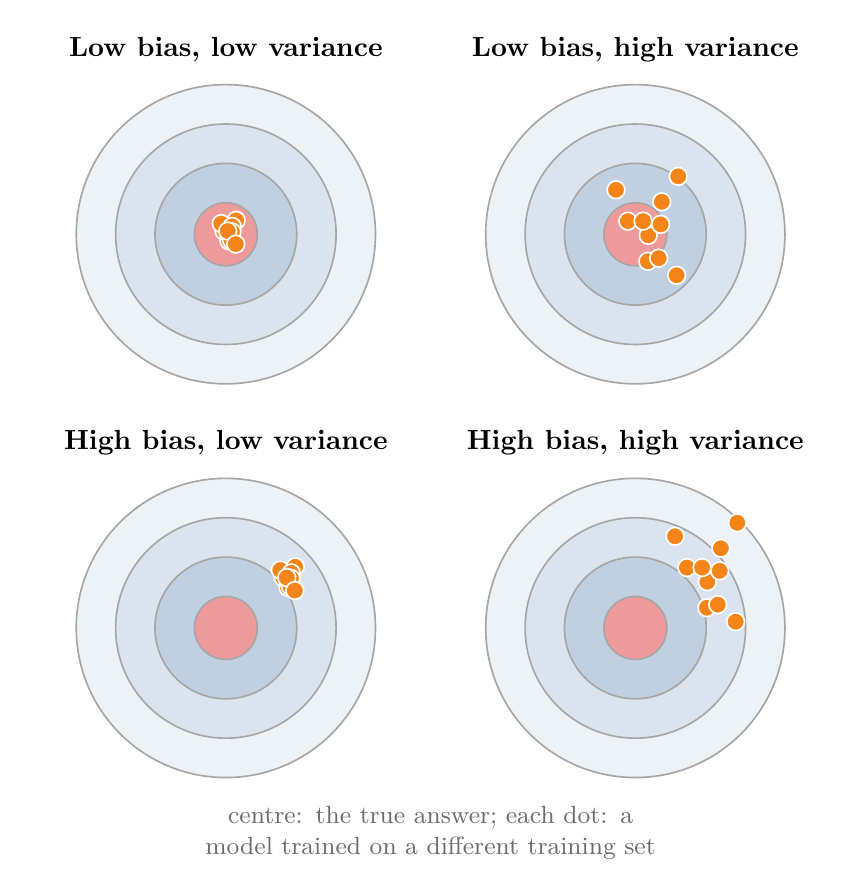
\begin{tikzpicture}
  \foreach \col/\row/\cx/\cy/\spread/\title in {0/0/0/0/0.18/{Low bias, low variance}, 1/0/0/0/0.75/{Low bias, high variance},
                                               0/1/0.75/0.6/0.18/{High bias, low variance}, 1/1/0.75/0.6/0.75/{High bias, high variance}} {
    \begin{scope}[shift={(\col*5.2,-\row*5)}]
      \foreach \r/\c in {1.9/cblue!10, 1.4/cblue!20, 0.9/cblue!35, 0.4/cred!60} \fill[\c] (0,0) circle (\r);
      \foreach \r in {1.9,1.4,0.9,0.4} \draw[cgrey!60, line width=0.6pt] (0,0) circle (\r);
      \pgfmathsetseed{7}
      \foreach \i in {1,...,10} {
        \pgfmathsetmacro{\px}{\cx + \spread*rand}
        \pgfmathsetmacro{\py}{\cy + \spread*rand}
        \fill[corange, draw=white, line width=0.6pt] (\px,\py) circle (3.2pt);
      }
      \node[font=\bfseries] at (0,2.35) {\title};
    \end{scope}
  }
  \node[note, text width=10cm] at (2.6,-7.6) {centre: the true answer; each dot: a model trained on a different training set};
\end{tikzpicture}
\end{document}
